\documentclass[../main.tex]{subfiles}





\begin{document}
\chapter{}
\label{cha:cha_19}

\section{}
\begin{enumerate}[label=\bfseries(\alph*)]
\item  Euler's method. Here are the first few steps
	\bigbreak
\begin{tabular}{rcclc}
\hline
\multicolumn{1}{c}{$t$} & $x$ & $y$ & $d x / d t$ & $d y / d t$ \\
\hline
0 & $2.0000$ & $1.0000$ & $1.2000$ & $-0.2000$ \\
$0.1$ & $2.1200$ & $0.9800$ & $1.2974$ & $-0.1607$ \\
$0.2$ & $2.2497$ & $0.9639$ & $1.3985$ & $-0.1206$ \\
$0.3$ & $2.3896$ & $0.9519$ & $1.5028$ & $-0.0791$ \\
$0.4$ & $2.5399$ & $0.9440$ & $1.6093$ & $-0.0359$ \\
$0.5$ & $2.7008$ & $0.9404$ & $1.7171$ & $0.0096$ \\
\hline
\end{tabular}
	\bigbreak
The computation can be continued and the results plotted versus time:
	\bigbreak
	\begin{figure}[H]
		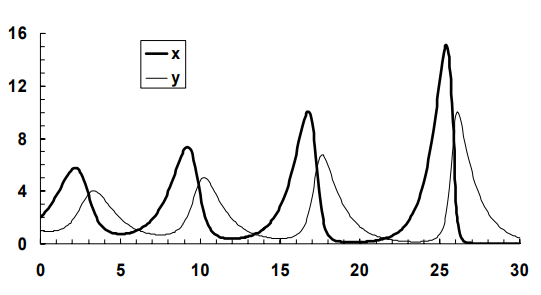
\includegraphics[width=0.5\linewidth]{fig_19_1}
		\label{fig:fig_19_1}
	\end{figure}
	\bigbreak
Notice that the amplitudes of the oscillations are expanding. This is also illustrated by a state-space plot ( $y$ versus $x$ ):
	\bigbreak
	\begin{figure}[H]
		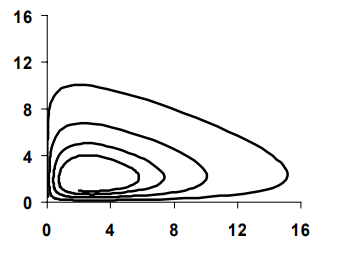
\includegraphics[width=0.5\linewidth]{fig_19_2}
		\label{fig:fig_19_2}
	\end{figure}
	\bigbreak
\item RK4. Here is the first step in detail.
	\bigbreak
$k_{1,1}=f_{1}(0,2,1)=1.5(2)-0.7(2)(1)=1.6$
	\bigbreak
$k_{1,2}=f_{2}(0,2,1)=-0.9(1)+0.4(2)(1)=-0.1$
	\bigbreak
$x(0.05)=2+1.6(0.05)=2.08 $
	\bigbreak
$y(0.05)=1-0.1(0.05)=0.995 $
	\bigbreak
$k_{2,1}=f_{1}(0.05,2.08,0.995)=1.67128 $
	\bigbreak
$k_{2,2}=f_{2}(0.05,2.08,0.995)=-0.06766 $
	\bigbreak
$x(0.05)=2+1.67128(0.05)=2.083564 $
	\bigbreak
$y(0.05)=1-9(0.05)=0.996617 $
	\bigbreak
$k_{3,1}=f_{1}(0.05,2.083564,0.996617)=1.671785 $
	\bigbreak
$k_{3,2}=f_{2}(0.05,2.083564,0.996617)=-0.06635 $
	\bigbreak
$x(0.1)=2+1.671785(0.1)=2.167179 $
	\bigbreak
$y(0.1)=1-0.06635(0.1)=0.993365 $
	\bigbreak
$k_{4,1}=f_{1}(0.1,2.167179,0.993365)=1.743808 $
	\bigbreak
$k_{4,2}=f_{2}(0.1,2.167179,0.993365)=-0.03291$
	\bigbreak
The $k$ 's can then be used to compute the increment functions,
	\bigbreak
$\phi_{1}=\dfrac{1.6+2(1.67128+1.671785)+1.743808}{6}=1.671656$
	\bigbreak
$\phi_{2}=\dfrac{-0.1+2(-0.06766-0.06635)-0.03291}{6}=-0.06682$
	\bigbreak
These slope estimates can then be used to make the prediction for the first step
	\bigbreak
$x(0.1)=2+1.671656(0.1)=2.16766$
	\bigbreak
$y(0.1)=1-0.06682(0.1)=0.993318$
	\bigbreak
The remaining steps can be taken in a similar fashion and the first few results summarized as
	\bigbreak
\begin{tabular}{rrr}
\hline
\multicolumn{1}{c}{$t$} & \multicolumn{1}{c}{$x$} & \multicolumn{1}{c}{$y$} \\
\hline
0 & 2 & 1 \\
$0.1$ & $2.167166$ & $0.993318$ \\
$0.2$ & $2.348838$ & $0.993588$ \\
$0.3$ & $2.545029$ & $1.001398$ \\
$0.4$ & $2.755314$ & $1.017509$ \\
$0.5$ & $2.978663$ & $1.042891$ \\
\hline
\end{tabular}
	\bigbreak
A plot of all the values can be developed. Note that in contrast to Euler's method, the cycles do not amplify as time proceeds.
	\bigbreak
	\begin{figure}[H]
		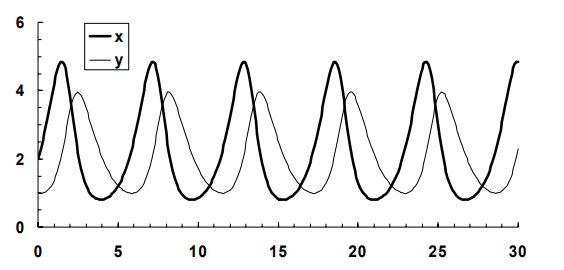
\includegraphics[width=0.5\linewidth]{fig_19_3}
		\label{fig:fig_19_3}
	\end{figure}
	\bigbreak
This periodic nature is also evident from the state-space plot. Because this is the expected behavior we can see that the RK4 is far superior to Euler's method for this particular problem.
	\bigbreak
	\begin{figure}[H]
		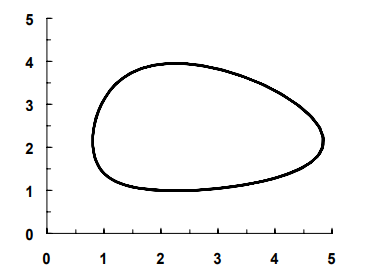
\includegraphics[width=0.5\linewidth]{fig_19_4}
		\label{fig:fig_19_4}
	\end{figure}
	\bigbreak
\item To implement ode45, first a function is developed to evaluate the predator-prey ODEs,
	\bigbreak
\begin{lstlisting}[numbers=none]
function yp = predprey(t,y)
yp = [1.5*y(1)-0.7*y(1)*y(2);-0.9*y(2)+0.4*y(1)*y(2)];
\end{lstlisting}
	\bigbreak
Then, the solution and plot can be obtained:
	\bigbreak
\begin{lstlisting}[numbers=none]
>> [t,y] = ode45(@predprey,[0 30],[2 1]);
>> plot(t,y(:,1),t,y(:,2),'--')
>> legend('x(prey)','y(predator)') 
\end{lstlisting}
	\bigbreak
	\begin{figure}[H]
		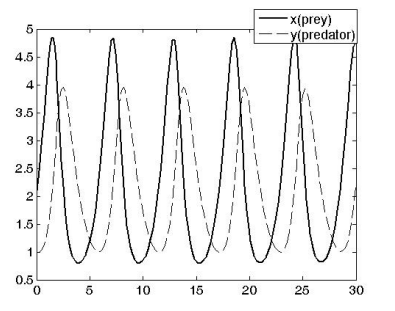
\includegraphics[width=0.5\linewidth]{fig_19_5}
		\label{fig:fig_19_5}
	\end{figure}
	\bigbreak
\end{enumerate}



\section{}
\begin{enumerate}[label=\bfseries(\alph*)]
\item Here are the results for the first few steps as computed with the classical RK4 technique
	\bigbreak
\begin{tabular}{rcrrr}
\multicolumn{1}{c}{$t$} & \multicolumn{1}{c}{$x$} & \multicolumn{1}{l}{$y$} & \multicolumn{1}{c}{$z$} \\
0 & 5 & 5 & 5 \\
$0.1$ & $9.78147$ & $17.07946$ & $10.43947$ \\
$0.2$ & $17.70297$ & $20.8741$ & $35.89688$ \\
$0.3$ & $10.81088$ & $-2.52924$ & $39.30744$ \\
$0.4$ & $0.549578$ & $-5.54419$ & $28.07462$ \\
$0.5$ & $-3.1646$ & $-5.84128$ & $22.36888$ \\
$0.6$ & $-5.57588$ & $-8.42037$ & $19.92312$ \\
$0.7$ & $-8.88719$ & $-12.6789$ & $22.14148$ \\
$0.8$ & $-11.9142$ & $-13.43$ & $29.80001$ \\
$0.9$ & $-10.6668$ & $-7.21784$ & $33.39903$ \\
1 & $-6.84678$ & $-3.43018$ & $29.30717$ \\
\end{tabular}
	\bigbreak
The results from $t=0$ to 20 can be displayed graphically as
	\bigbreak
	\begin{figure}[H]
		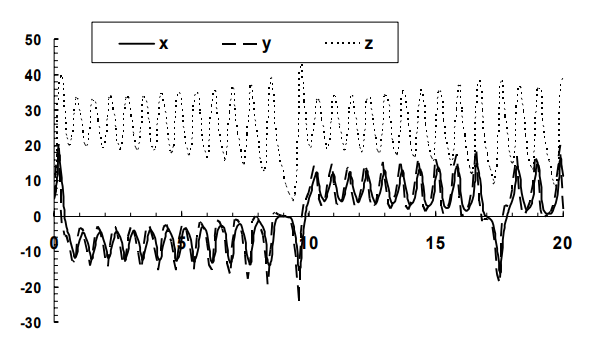
\includegraphics[width=0.5\linewidth]{fig_19_6}
		\label{fig:fig_19_6}
	\end{figure}
	\bigbreak
The solution appears chaotic bouncing around from negative to positive values. Although the pattern might appear random, an underlying pattern emerges when we look at the statespace plots. For example, here is the plot of $y$ versus $x$.
	\bigbreak
	\begin{figure}[H]
		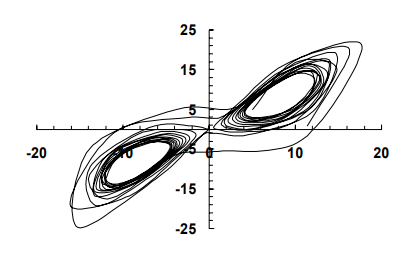
\includegraphics[width=0.5\linewidth]{fig_19_7}
		\label{fig:fig_19_7}
	\end{figure}
	\bigbreak
And here is $z$ versus $x$,
	\bigbreak
	\begin{figure}[H]
		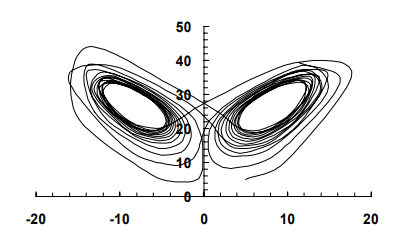
\includegraphics[width=0.5\linewidth]{fig_19_8}
		\label{fig:fig_19_8}
	\end{figure}
	\bigbreak
\item To implement any of the MATLAB functions, first a function is developed to evaluate the Lorenz ODEs,
	\bigbreak
\begin{lstlisting}[numbers=none]
function yp = lorenz(t,y)
yp = [-10*y(1)+10*y(2);28*y(1)-y(2)-y(1)*y(3);-2.666667*y(3)+y(1)*y(2)]; 
\end{lstlisting}
	\bigbreak
Then, the solution and plots for the ode 23 function can be obtained:
	\bigbreak
\begin{lstlisting}[numbers=none]
>> [t,y] = ode23(@lorenz,[0 20],[5 5 5]);
>> plot(t,y(:,1),t,y(:,2),'--',t,y(:,3),':')
>> legend('x','y','z')
>> plot(y(:,1),y(:,2))
\end{lstlisting}
	\bigbreak
	\begin{figure}[H]
		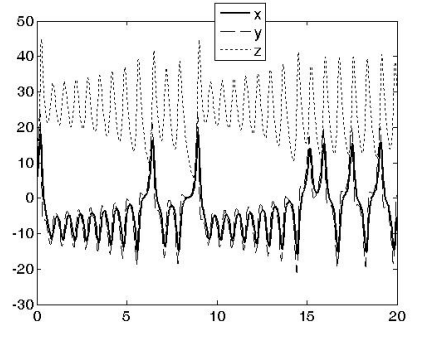
\includegraphics[width=0.5\linewidth]{fig_19_9}
		\label{fig:fig_19_9}
	\end{figure}
	\bigbreak
Notice how this plot, although qualitatively similar to the constant step RK4 result in (a), the details are quite different. However, the state-space representation looks much more consistent.
	\bigbreak
\begin{lstlisting}[numbers=none]
>> plot(y(:,1),y(:,2))
\end{lstlisting}
	\bigbreak
	\begin{figure}[H]
		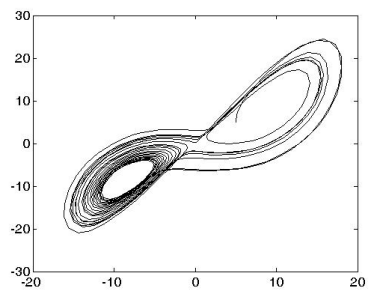
\includegraphics[width=0.5\linewidth]{fig_19_10}
		\label{fig:fig_19_10}
	\end{figure}
	\bigbreak
\item The ode 45 again differs in the details of the time-series plot,
	\bigbreak
\begin{lstlisting}[numbers=none]
>> [t,y] = ode45(@lorenz,[0 20],[5 5 5]);
>> plot(t,y(:,1),t,y(:,2),'--',t,y(:,3),':')
>> legend('x','y','z') 
\end{lstlisting}
	\bigbreak
	\begin{figure}[H]
		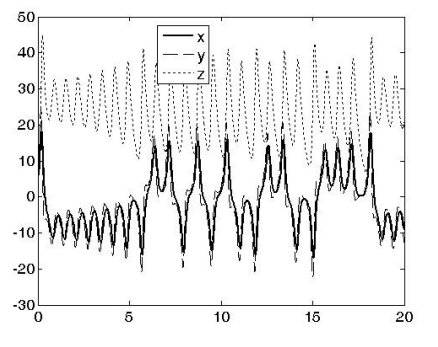
\includegraphics[width=0.5\linewidth]{fig_19_11}
		\label{fig:fig_19_11}
	\end{figure}
	\bigbreak
\item The ode23tb also differs in the details of the time-series plot,
	\bigbreak
\begin{lstlisting}[numbers=none]
>> [t,y] = ode23tb(@lorenz,[0 20],[5 5 5]);
>> plot(t,y(:,1),t,y(:,2),'--',t,y(:,3),':')
>> legend('x','y','z') 
\end{lstlisting}
	\bigbreak
	\begin{figure}[H]
		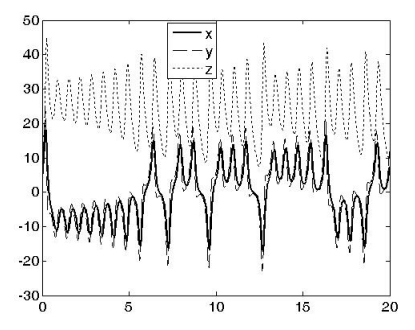
\includegraphics[width=0.5\linewidth]{fig_19_12}
		\label{fig:fig_19_12}
	\end{figure}
	\bigbreak
\begin{blockquote}
Close inspection of all the above results indicates that they all yield identical results for a period of time. Thereafter, they abruptly begin to diverge. The reason for this behavior is that these equations are highly sensitive to their initial conditions. After a number of steps, because they all employ different algorithms, they begin to diverge slightly. When the discrepancy becomes large enough (which for these equations is not that much), the solution will tend to make a large jump. Thus, after awhile, the various solutions become uncorrelated. Such solutions are said to be chaotic. It was this characteristic of these particular equations that led Lorenz to suggest that long-range weather forecasts might not be possible.
\end{blockquote}
	\bigbreak
\end{enumerate}




\section{}
First step:
	\bigbreak
Predictor:
	\bigbreak
$y_{1}^{0}=5.222138+\left[-0.5(4.143883)+e^{-2}\right] 1=3.285532$
	\bigbreak
Corrector:
	\bigbreak
$y_{1}^{1}=4.143883+\dfrac{-0.5(4.143883)+e^{-2}-0.5(3.285532)+e^{-2.5}}{2} 0.5=3.269562$
	\bigbreak
The corrector can be iterated to yield
	\bigbreak
$
\begin{array}{ccc}
j & y_{i+1}^{j} & \left|\varepsilon_{a}\right|, \% \\ 
1 & 3.269562 & \\
 2 & 3.271558 & 0.061
\end{array}
$
	\bigbreak
Second step:
	\bigbreak
Predictor:
	\bigbreak
$y_{2}^{0}=4.143883+\left[-0.5(3.271558)+e^{-2.5}\right] 1=2.590189$
	\bigbreak
Predictor Modifier:
	\bigbreak
$y_{2}{ }^{0}=2.590189+4 / 5(3.271558-3.285532)=2.579010$
	\bigbreak
Corrector:
	\bigbreak
$y_{2}{ }^{1}=3.271558+\dfrac{-0.5(3.271558)+e^{-2.5}-0.5(2.579010)+e^{-3}}{2} 0.5=2.573205$
	\bigbreak
The corrector can be iterated to yield
	\bigbreak
$
\begin{array}{ccc}
j & y_{i+1}^{j} & \left|\varepsilon_{a}\right|, \% \\
1 & 2.573205 & \\
2 & 2.573931 & 0.0282
\end{array}
$
	\bigbreak




\section{}
Before solving, for comparative purposes, we can develop the analytical solution as
	\bigbreak
$y=e^{\dfrac{t^{3}}{3}-t}$
	\bigbreak
Thus, the true values being simulated in this problem are
	\bigbreak
\begin{tabular}{rr}
\hline
\multicolumn{1}{c}{$t$} & \multicolumn{1}{c}{$y$} \\
\hline
0 & 1 \\
$0.25$ & $0.782868$ \\
$0.5$ & $0.632337$ \\
\hline
\end{tabular}
	\bigbreak
The first step is taken with the fourth-order RK:
	\bigbreak
$k_{1}=f(0,1)=1(0)^{2}-1=-1$
	\bigbreak
$y(0.125)=1-1(0.125)=0.875$
	\bigbreak 
$k_{2}=f(0.125,0.875)=-0.861328$
	\bigbreak 
$y(0.125)=1-0.861328(0.125)=0.89233$
	\bigbreak
$k_{3}=f(0.125,0.89233)=-0.87839$
	\bigbreak
$y(0.25)=1-0.87839(0.25)=0.78040$
	\bigbreak
$k_{4}=f(0.25,0.78040)=-0.73163$
	\bigbreak
$\phi=\dfrac{-1+2(-0.861328-0.87839)-0.73163}{6}=-0.86851$
	\bigbreak
$y(0.25)=1-0.86851(0.25)=0.7828723$
	\bigbreak
This result compares favorably with the analytical solution.
	\bigbreak
The second step can then be implemented with the non-self-starting Heun method:
	\bigbreak
Predictor:
	\bigbreak
$y(0.5)=1+\left(0.7828723(0.25)^{2}-0.7828723\right) 0.5=0.633028629$
	\bigbreak
Corrector: (First iteration):
	\bigbreak
$y(0.5)=0.7828723+\dfrac{-0.7339+\left(0.633028629(0.5)^{2}-0.633028629\right)}{2} 0.25=0.63178298$
	\bigbreak
Corrector: (Second iteration):
	\bigbreak
$y(0.5)=0.7828723+\dfrac{-0.7339+\left(0.63178298(0.5)^{2}-0.63178298\right)}{2} 0.25=0.63189976$
	\bigbreak
The iterative process can be continued with the final result converging on $0.63188975 .$



\section{}
\begin{enumerate}[label=\bfseries(\alph*)]
\item $h<2 / 100,000=2 \times 10^{-5}$.
	\bigbreak
\item The implicit Euler can be written for this problem as
	\bigbreak
$y_{i+1}=y_{i}+\left(-100,000 y_{i+1}+99,999 e^{-t_{i+1}}\right) h$
	\bigbreak
which can be solved for
	\bigbreak
$y_{i+1}=\dfrac{y_{i}+99,999 e^{-t_{i+1}} h}{1+100,000 h}$
	\bigbreak
The results of applying this formula for the first few steps are shown below. A plot of the entire solution is also displayed
	\bigbreak
\begin{tabular}{rr}
\hline
$t$ & $y$ \\
\hline
0 & 0 \\
$0.1$ & $1.904638$ \\
$0.2$ & $1.818731$ \\
$0.3$ & $1.740819$ \\
$0.4$ & $1.67032$ \\
$0.5$ & $1.606531$ \\
\hline
\end{tabular}
	\bigbreak
	\begin{figure}[H]
		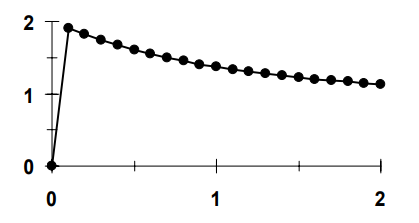
\includegraphics[width=0.5\linewidth]{fig_19_13}
		\label{fig:fig_19_13}
	\end{figure}
	\bigbreak
\end{enumerate}



\section{}
The implicit Euler can be written for this problem as
	\bigbreak
$y_{i+1}=y_{i}+\left(30\left(\sin t_{i+1}-y_{i+1}\right)+3 \cos t_{i+1}\right) h$
	\bigbreak
which can be solved for
	\bigbreak
$y_{i+1}=\dfrac{y_{i}+30 \sin t_{i+1} h+3 \cos t_{i+1} h}{1+30 h}$
	\bigbreak
The results of applying this formula are tabulated and graphed below.
	\bigbreak
\begin{tabular}{rrrrrrrr}
\hline
\multicolumn{1}{c}{$\boldsymbol{t}$} & $\boldsymbol{y}$ & $\boldsymbol{t}$ & $\boldsymbol{y}$ & $\boldsymbol{t}$ & $\boldsymbol{y}$ & $\boldsymbol{t}$ & $\boldsymbol{y}$ \\
\hline
0 & 0 & $1.2$ & $0.952306$ & $2.4$ & $0.622925$ & $3.6$ & $-0.50089$ \\
$0.4$ & $0.444484$ & $1.6$ & $0.993242$ & $2.8$ & $0.270163$ & 4 & $-0.79745$ \\
$0.8$ & $0.760677$ & 2 & $0.877341$ & $3.2$ & $-0.12525$ &  &  \\
\hline
\end{tabular}
	\bigbreak
	\begin{figure}[H]
		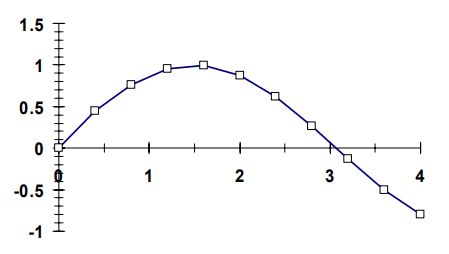
\includegraphics[width=0.5\linewidth]{fig_19_14}
		\label{fig:fig_19_14}
	\end{figure}
	\bigbreak



\section{}
\begin{enumerate}[label=\bfseries(\alph*)]
\item The explicit Euler can be written for this problem as
	\bigbreak
$x_{1, i+1}=x_{1, i}+\left(999 x_{1, i}+1999 x_{2, i}\right) h$
	\bigbreak
$x_{2, i+1}=x_{2, i}+\left(-1000 x_{1, i}-2000 x_{2, i}\right) h$
	\bigbreak
Because the step-size is much too large for the stability requirements, the solution is unstable,
	\bigbreak
\begin{tabular}{rrrrr}
\hline
\multicolumn{1}{c}{$t$} & \multicolumn{1}{c}{$x_{1}$} & \multicolumn{1}{c}{$x_{2}$} & $d x_{1} / d t$ & $d x 2 / d t$ \\
\hline
0 & 1 & 1 & 2998 & $-3000$ \\
$0.05$ & $150.9$ & $-149$ & $-147102$ & 147100 \\
$0.1$ & $-7204.2$ & 7206 & 7207803 & $-7207805$ \\
$0.15$ & 353186 & $-353184$ & $-3.5 E+08$ & $3.53 E+08$ \\
$0.2$ & $-1.7 E+07$ & 17305943 & $1.73 E+10$ & $-1.7 E+10$ \\
\hline
\end{tabular}
	\bigbreak
\item The implicit Euler can be written for this problem as
	\bigbreak
$x_{1, i+1}=x_{1, i}+\left(999 x_{1, i+1}+1999 x_{2, i+1}\right) h$
	\bigbreak
$x_{2, i+1}=x_{2, i}+\left(-1000 x_{1, i+1}-2000 x_{2, i+1}\right) h$
	\bigbreak
or collecting terms
	\bigbreak
$(1-999 h) x_{1, i+1}-1999 h x_{2, i+1}=x_{1, i}$
	\bigbreak
$1000 h x_{1, i+1}+(1+2000 h) x_{2, i+1}=x_{2, i}$
	\bigbreak
or substituting $h=0.05$ and expressing in matrix format
	\bigbreak
$
\left[\begin{array}{cc}
-48.95 & -99.95 \\
50 & 101
\end{array}\right]\left\{\begin{array}{l}
x_{1, i+1} \\
x_{2, i+1}
\end{array}\right\}=\left\{\begin{array}{l}
x_{1, i} \\
x_{2, i}
\end{array}\right\}
$
	\bigbreak
\begin{blockquote}
Thus, to solve for the first time step, we substitute the initial conditions for the right-hand side and solve the $2 x 2$ system of equations. The best way to do this is with LU decomposition since we will have to solve the system repeatedly. For the present case, because its easier to display, we will use the matrix inverse to obtain the solution. Thus, if the matrix is inverted, the solution for the first step amounts to the matrix multiplication,
\end{blockquote}
	\bigbreak
$
\left\{\begin{array}{l}
x_{1, i+1} \\
x_{2, i+1}
\end{array}\right\}=\left[\begin{array}{cc}
1.886088 & 1.86648 \\
-0.93371 & -0.9141
\end{array}\right]\{1\}=\left\{\begin{array}{c}
3.752568 \\
-1.84781
\end{array}\right\}
$
	\bigbreak
For the second step (from $x=0.05$ to $0.1)$,
	\bigbreak
$
\left\{\begin{array}{l}
x_{1, i+1} \\
x_{2, i+1}
\end{array}\right\}=\left[\begin{array}{cc}
1.886088 & 1.86648 \\
-0.93371 & -0.9141
\end{array}\right]\left\{\begin{array}{c}
3.752568 \\
-1.84781
\end{array}\right\}=\left\{\begin{array}{c}
3.62878 \\
-1.81472
\end{array}\right\}
$
	\bigbreak
The remaining steps can be implemented in a similar fashion to give
	\bigbreak
\begin{tabular}{rrr}
\hline
$\boldsymbol{t}$ & $\boldsymbol{x}_{\mathbf{1}}$ & $\boldsymbol{x}_{\mathbf{2}}$ \\
\hline
0 & 1 & 1 \\
$0.05$ & $3.752568$ & $-1.84781$ \\
$0.1$ & $3.62878$ & $-1.81472$ \\
$0.15$ & $3.457057$ & $-1.72938$ \\
$0.2$ & $3.292457$ & $-1.64705$ \\
\hline
\end{tabular}
	\bigbreak
The results are plotted below, along with a solution with the explicit Euler using a step of $0.0005$.
	\bigbreak
	\begin{figure}[H]
		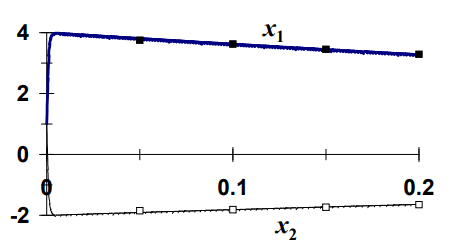
\includegraphics[width=0.5\linewidth]{fig_19_15}
		\label{fig:fig_19_15}
	\end{figure}
	\bigbreak
\end{enumerate}



\section{}
\begin{enumerate}[label=\bfseries(\alph*)]
\item The exact solution is
	\bigbreak
$y=A e^{5 t}+t^{2}+0.4 t+0.08$
	\bigbreak
If the initial condition at $t=0$ is $0.8, A=0$,
	\bigbreak
$y=t^{2}+0.4 t+0.08$
	\bigbreak
\begin{blockquote}
Note that even though the choice of the initial condition removes the positive exponential terms, it still lurks in the background. Very tiny round off errors in the numerical solutions bring it to the fore. Hence all of the following solutions eventually diverge from the analytical solution.
\end{blockquote}
	\bigbreak
\item $4^{\text {th }}$ order RK. The plot shows the numerical solution (bold line) along with the exact solution (fine line).
	\bigbreak
	\begin{figure}[H]
		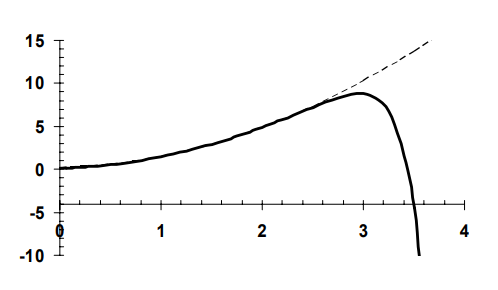
\includegraphics[width=0.5\linewidth]{fig_19_16}
		\label{fig:fig_19_16}
	\end{figure}
	\bigbreak
\item
	\bigbreak
\begin{lstlisting}[numbers=none]
function yp = dy(t,y)
yp = 5*(y-t^2);


>> tspan = [0,5];
>> y0 = 0.08;
>> [t,y] = ode45(@dy1,tspan,y0); 
\end{lstlisting}
	\bigbreak
\item
	\bigbreak
\begin{lstlisting}[numbers=none]
>> [t,y] = ode23s(@dy1,tspan,y0); 
\end{lstlisting}
	\bigbreak
\item
	\bigbreak
\begin{lstlisting}[numbers=none]
>> [t,y] = ode23tb(@dy1,tspan,y0);
\end{lstlisting}
	\bigbreak
	\begin{figure}[H]
		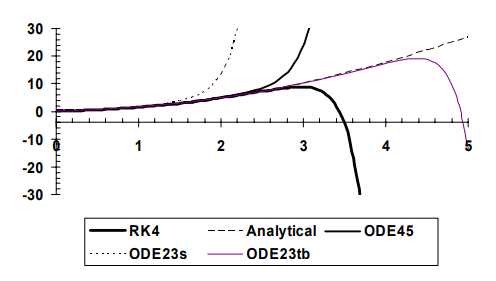
\includegraphics[width=0.5\linewidth]{fig_19_17}
		\label{fig:fig_19_17}
	\end{figure}
\end{enumerate}



\section{}
\begin{enumerate}[label=\bfseries(\alph*)]
\item As in Example 17.5, the humps function can be integrated with the quad function as in
	\bigbreak
\begin{lstlisting}[numbers=none]
>> format long
>> quad(@humps,0,1)


ans =
 	29.85832612842764 
\end{lstlisting}
	\bigbreak
\item Using ode 45 is based on recognizing that the evaluation of the definite integral
	\bigbreak
$\displaystyle I=\int_{a}^{b} f(x) d x$
	\bigbreak
is equivalent to solving the differential equation
	\bigbreak
$\dfrac{d y}{d x}=f(x)$
	\bigbreak
for $y(b)$ given the initial condition $y(a)=0$. Thus, we must solve the following initial-value problem:
	\bigbreak
$\dfrac{d y}{d x}=\dfrac{1}{(x-0.3)^{2}+0.01}+\dfrac{1}{(x-0.9)^{2}+0.04}-6$
	\bigbreak
where $y(0)=0$. To do this with ode45, we must first set up an M-file to evaluate the righthand side of the differential equation,
	\bigbreak
\begin{lstlisting}[numbers=none]
function dy = humpsODE(x,y)
dy = 1./((x-0.3).^2 + 0.01) + 1./((x-0.9).^2+0.04) - 6;
\end{lstlisting}
	\bigbreak
Then, the integral can be evaluated as 
	\bigbreak
\begin{lstlisting}[numbers=none]
>> [x,y] = ode45(@humpsODE,[0 0.5 1],0);
>> disp([x,y])
 			        0 				0
 	0.50000000000000 	21.78356481821654
 	1.00000000000000 	29.85525185285369 
\end{lstlisting}
	\bigbreak
Thus, the integral estimate is within $0.01 \%$ of the estimate obtained with the quad function. Note that a better estimate can be obtained by using the odeset function to set a smaller relative tolerance as in
	\bigbreak
\end{enumerate}



\section{}
The nonlinear model can be expressed as the following set of ODEs,
	\bigbreak
$\dfrac{d \theta}{d t}=v$
	\bigbreak
$\dfrac{d v}{d t}=-\dfrac{g}{l} \sin \theta$
	\bigbreak
where $v=$ the angular velocity. A function can be developed to compute the right-hand-side of this pair of ODEs for the case where $g=9.81$ and $l=0.6 \mathrm{~m}$,
	\bigbreak
\begin{lstlisting}[numbers=none]
function dy = dpnon(t, y)
dy = [y(2);-9.81/0.6*sin(y(1))];
\end{lstlisting}
	\bigbreak
The linear model can be expressed as the following set of ODEs,
	\bigbreak
$\dfrac{d \theta}{d t}=v$
	\bigbreak
$\dfrac{d v}{d t}=-\dfrac{g}{l}$
	\bigbreak
A function can be developed as,
	\bigbreak
\begin{lstlisting}[numbers=none]
function dy = dplin(t, y)
dy = [y(2);-9.81/0.6*y(1)];
\end{lstlisting}
	\bigbreak
Then, the solution and plot can be obtained for the case where $\theta(0)=\pi / 8$. Note that we only depict the displacement $(\theta$ or $\mathrm{y}(1))$ in the plot
	\bigbreak
\begin{lstlisting}[numbers=none]
>> [tn yn] = ode45(@dpnon,[0 10],[pi/8 0]);
>> [tl yl] = ode45(@dplin,[0 10],[pi/8 0]);
>> plot(tn,yn(:,1),tl,yl(:,1),'--')
>> legend('nonlinear','linear') 
\end{lstlisting}
	\bigbreak
	\begin{figure}[H]
		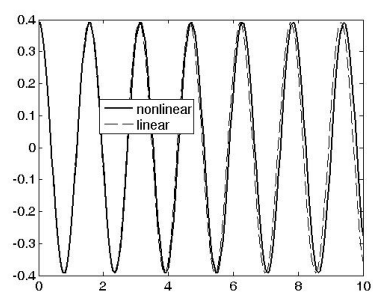
\includegraphics[width=0.5\linewidth]{fig_19_18}
		\label{fig:fig_19_18}
	\end{figure}
	\bigbreak
\begin{blockquote}
You should notice two aspects of this plot. First, because the displacement is small, the linear solution provides a decent approximation of the more physically realistic nonlinear case. Second, the two solutions diverge as the computation progresses.
\end{blockquote}
	\bigbreak
For the larger initial displacement $(\theta(0)=\pi / 8)$, the solution and plot can be obtained as,
	\bigbreak
\begin{lstlisting}[numbers=none]
>> [tn yn] = ode45(@dpnon,[0 10],[pi/2 0]);
>> [tl yl] = ode45(@dplin,[0 10],[pi/2 0]);
>> plot(tn,yn(:,1),tl,yl(:,1),'--')
>> legend('nonlinear','linear') 
\end{lstlisting}
	\bigbreak
	\begin{figure}[H]
		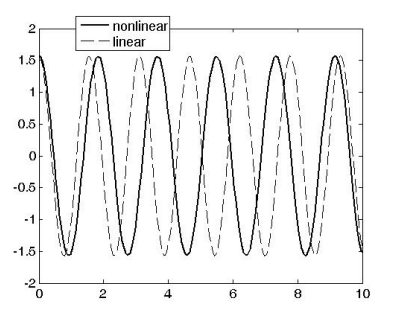
\includegraphics[width=0.5\linewidth]{fig_19_19}
		\label{fig:fig_19_19}
	\end{figure}
	\bigbreak
\begin{blockquote}
Because the linear approximation is only valid at small displacements, there are now clear and significant discrepancies between the nonlinear and linear cases that are exacerbated as the solution progresses.
\end{blockquote}
	\bigbreak



\section{}
A function can be developed to compute the right-hand-side of the ODE,
	\bigbreak
\begin{lstlisting}[numbers=none]
function yp = dpdt(t, p)
yp = 0.026*(1-p/12000)*p;
\end{lstlisting}
	\bigbreak
\begin{blockquote}
The function ode45 can be used to integrate this equation and generate results corresponding to the dates for the measured population data. A plot can also be generated of the solution and the data
\end{blockquote}
	\bigbreak
\begin{lstlisting}[numbers=none]
>> tspan = 1950:5:2000;
>> pdata = [2555 2780 3040 3346 3708 4087 4454 4850 5276 5686 6079]';
>> [t,p] = ode45(@dpdt,tspan,2555);
>> plot(t,p,t,pdata,'o') 
\end{lstlisting}
	\bigbreak
	\begin{figure}[H]
		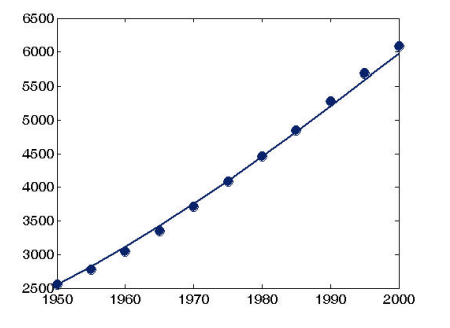
\includegraphics[width=0.5\linewidth]{fig_19_20}
		\label{fig:fig_19_20}
	\end{figure}
	\bigbreak
The sum of the squares of the residuals can be computed as
	\bigbreak
\begin{lstlisting}[numbers=none]
>> SSR = sum((p - pdata).^2)


SSR =
	4.2365e+004
\end{lstlisting}
	\bigbreak
	\bigbreak
	\bigbreak
	\bigbreak
	\bigbreak
	\bigbreak
	\bigbreak
	\bigbreak
	\bigbreak
	\bigbreak
	\bigbreak
	\bigbreak
	\bigbreak
	\bigbreak
	\bigbreak
	\bigbreak
	\bigbreak
	\bigbreak
	\bigbreak
	\bigbreak
\end{document}